\documentclass[man]{apa}
\usepackage{graphicx}
\usepackage{pdfpages}
\usepackage{fullpage}
\usepackage[english]{babel}
\usepackage{amsmath}
\usepackage{apacite}
\usepackage{url}
%Kopf- und Fußzeile
\usepackage{fancyhdr}
%\pagestyle{fancy}
%\fancyhf{}
%Kopfzeile links bzw. innen
\shorttitle{Weight of social information}
\renewcommand{\headrulewidth}{0pt}
\title{Integrating social and individual information across the life span.}
\author{Julia Rodriguez-Buritica, Hauke Heekeren, Ray Dolan, Ulf Toelch}
\abstract{}
\affiliation{Mind and Brain \\ Humboldt University}
%\renewcommand{\figurename}{ESM Figure}
%\renewcommand{\tablename}{ESM Table}
\usepackage{hhline}
\begin{document}
\maketitle
\section{Introduction}

\section{General Methods}
\subsubsection{Experimental Game}
The game consisted of an initial training phase (15 trials) and two experimental phases (60 and 120 trials). The training phase and first phase involved guessing the location of a stimulus that briefly flashed on the screen whereas in the second phase players had to make a second guess based on their guesses from the first phase. 

\subsubsection{Training phase and first experimental phase}
Each trial was commenced by pressing a key and after an initial 1 s break a stimulus (filled circle) was briefly flashed for a short time interval (50 ms) on the outline of a pre-drawn circle on a computer screen. Immediately after the stimulus presentation distractor stimuli are displayed on the outline of the empty circle for 3 s. Participants then had to make a guess where on the outer empty circle the stimulus appeared. The location of their guess was displayed as a small red circle. In the first experimental phase players will see, additional to their own choice, a green and a yellow circle representing the choices of two other players. Experimental manipulation regarding those two players differed between experiments and details can be found in the respective sections. 
\subsubsection{Second Experimental Phase}
Each trial was started after a 1 s inter trial interval. In this phase players viewed choices from randomized trials from the first experimental phase. They always received two pieces of information to inform a second guess on where the stimulus was located. There were three information pairs; players saw their own guess paired with a guess from one of the two social players or they saw the two guesses from the social players but not their own. Players were given 8 s to make their choice. After they decided, a large cross appeared at the center of the screen. We excluded all trials from analysis (~4\%)  where players did not choose in time.

\section{Experiment 1}
\subsection{Method}
\subsubsection{Participants}
Twenty kids and 18 adolescents participated in this experiment (kids age min/max/average; adolescents age min/max/average). Before beginning, verbal instructions were given accompanied by a presentation and written informed consent was obtained from all participants. After the experiment, participants were paid in private and were debriefed. The procedures and questionnaires were approved by the \textbf{FILL IN ETHICS!!} and comply with the ethical guidelines of the APA.
\subsection{Experimental manipulation}
For each session, we invited two same sex participants and paired them with an adult model of the same sex. \textbf{FILL DETAILS ON MODEL CONSISTENCY.} We told participants that they would see the choices of the other two players in their session. That is, participants saw information from their peer (kid respectively adolescent) and an adult. We also showed pictures framed by the other players circle colour in the top corners of the screen to avoid confusion regarding the colours. The information from the other players was, however, manipulated so that both players had the same accuracy ($deviation=9 degree$). Actual deviations were calculated beforehand by drawing from a normal distribution ($\mu=0, sd=12$). The same deviations were then randomly distributed across trials so that social players had different choices each trial but were overall equally accurate. No subject raised any suspicion about this manipulation.

\begin{figure}
%\includegraphics[width=0.5\textwidth]{Figure_Methods}
%\caption{In phase 1 (80 trials) players assessed their own accuracy and the accuracy of the other players in a perceptual task where they had to guess the position of a briefly flashed stimulus. After observing the stimulus for 50 ms players several distractor stimuli appeared in quick succession in random places along a circle. During the whole time players had to center their mouse pointer that was slowly moved by the computer in one direction. After this players had to guess the position of the stimulus and then saw the decisions of two other players as well as the actual position of the stimulus. In phase 2 players received information from phase 1. They always saw a combination of two guesses consisting of either individual information (red) or social information (green, yellow). Based on this information players made a second guess on the position of the stimulus. In the second phase players received no feedback.}
\end{figure}
\subsubsection{Data Analysis}
The (Bayes) optimal solution when integrating multiple information sources is to weigh information by it's reliability. In this case, the reliability is given by the inverse variance of player accuracy that could be learned during phase 1 of the experiment. In phase 2, the deviation of the final guess from the initial guess (from phase 1) is weighted ($\omega$) by this accuracy. If players accurately estimated the accuracy of the social ($acc_{soc}$) and individual ($acc_{ind}$) information the Bayes optimal decision is given by Equation \ref{eq:M1} with Equation \ref{eq:M2a}. More weight is given to individual information when the accuracy of the social players is low. \\
We then calculated for each player the weight for social information (ranging from 0 to 1) that corresponds to a Bayes optimal choice given their own accuracy. This weight was equal for both the adult and peer model. In trials when they saw information from the two other players the expected deviation was 0.5 since both players had the same accuracy. In this case, the optimal decision was to place the choice in the second phase in the middle between the two points. \\
Deviations from Bayes optimality denote a bias for either individual information or the information provided by the demonstrators. Previous studies have already shown that this bias also depends on the accuracy of indivdual information (ToelchSCAN). To asess this bias, we calculated a linear regression (intercept set to 0) for each player for each of the three information treatments (Individual - Peer, Individual - Adult, Peer- Adult). As dependent variable, we used the distance between the individual estimate from phase 1 and the final decision in phase 2 and the distance between the two points initially provided as independent variable. That is, we determined the empirical $\omega$ from Equation \ref{eq:M1} whereas the Bayes optimal weight gives an expectation for a theoretically optimal estimate of $\omega$. Substratcting the slope of the regression from the Bayes optimal expectation will thus yield an individual estimate for the bias of each individual. 

\begin{equation}
D_{ind-fin}=\omega * D_{ind-soc}
\label{eq:M1}
\end{equation} 
\begin{equation}
\omega=\frac{acc_{ind}}{acc_{ind}+acc_{soc}}
\label{eq:M2a}
\end{equation}
\subsection{Questionnaire and psychological scales}

\section{Results}

In phase 1 adolescents achieved higher accuracy scores cmpared to the kids group (\ref{fig:F1}).

\begin{figure}[h]
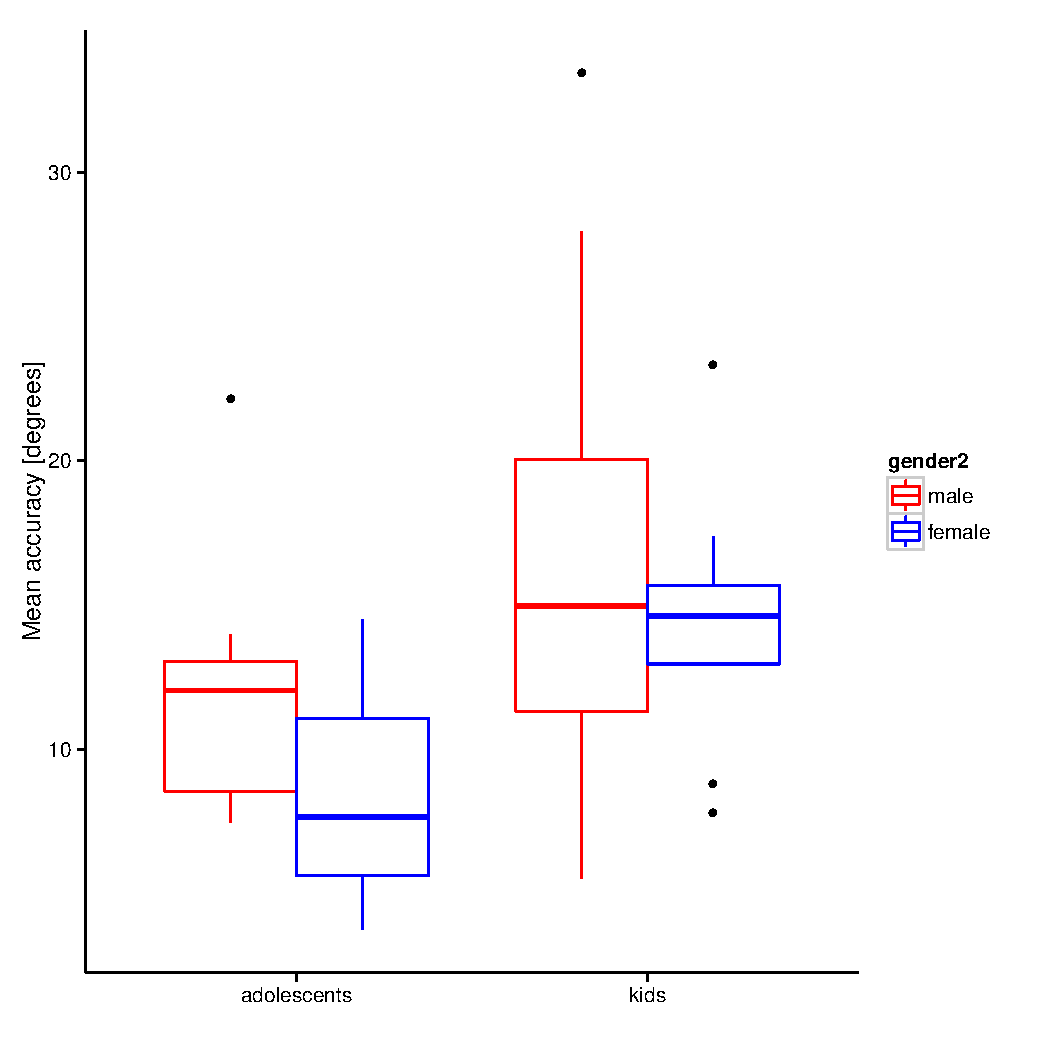
\includegraphics{Figure_1}
\caption{}
\label{fig:F1}
\end{figure}



\end{document}